\documentclass{tufte-handout}

%\geometry{showframe}% for debugging purposes -- displays the margins

\usepackage{amsmath}


% Set up the images/graphics package
\usepackage{graphicx}
\setkeys{Gin}{width=\linewidth,totalheight=\textheight,keepaspectratio}
\graphicspath{{graphics/}}


% The following package makes prettier tables.  We're all about the bling!
\usepackage{booktabs}

% The units package provides nice, non-stacked fractions and better spacing
% for units.
\usepackage{units}

% The fancyvrb package lets us customize the formatting of verbatim
% environments.  We use a slightly smaller font.
\usepackage{fancyvrb}
\fvset{fontsize=\normalsize}

% Small sections of multiple columns
\usepackage{multicol}

% Provides paragraphs of dummy text
\usepackage{lipsum}

\usepackage{lettrine} % The lettrine is the first enlarged letter at the beginning of the text

% These commands are used to pretty-print LaTeX commands
\newcommand{\doccmd}[1]{\texttt{\textbackslash#1}}% command name -- adds backslash automatically
\newcommand{\docopt}[1]{\ensuremath{\langle}\textrm{\textit{#1}}\ensuremath{\rangle}}% optional command argument
\newcommand{\docarg}[1]{\textrm{\textit{#1}}}% (required) command argument
\newenvironment{docspec}{\begin{quote}\noindent}{\end{quote}}% command specification environment
\newcommand{\docenv}[1]{\textsf{#1}}% environment name
\newcommand{\docpkg}[1]{\texttt{#1}}% package name
\newcommand{\doccls}[1]{\texttt{#1}}% document class name
\newcommand{\docclsopt}[1]{\texttt{#1}}% document class option name


%%% Additions to template by DSL
\usepackage{hyperref} % provides \url{}
% remove separation between list items http://tex.stackexchange.com/a/10689/1783
\usepackage{enumitem}
\setlist{nosep}


\title{Emergence in Network Automata}
\author{Richard Foard}
\date{7 October 2018}  % if the \date{} command is left out, the current date will be used
\begin{document}

\maketitle% this prints the handout title, author, and date
\marginnote{\textsc{Contact:\\
David LeBauer\\
email: dlebauer@gmail.com\\
phone: 919-275-0360
}}


\begin{abstract}
\noindent A simple, rule-based
graph automaton was defined and simulated. Each of its possible rules specifies a set
of local topology and node state changes to be applied iteratively, starting with a random initial graph.
Simulation runs were performed using many different rules, each run terminating when its graph
collapsed or cycled.
Evolving and terminal graph states were analyzed macroscopically, using
aggregate statistics, and microscopically, by inspecting graph structures.
Results were compared with those from simulations of a machine that
iterated by applying random, rather than rule-based, changes. We found that...
\end{abstract}

\section{Fungal Ecology \&  Physiology}

\subsection{The Carbon Cycle: Plants and Fungi}

\newthought{Since Alan Turing conceived his
universal machine} in 1936, simple abstract automata have drawn research attention.
Interest broadened beyond the academic realm in 1970,
when Conway published his \textit{Game of Life} simulations [citation needed] that highlighted the ability
of uncomplicated cellular automata to behave in complex ways. Researchers in the
nascent field of complexity theory began studying similar phenomena, such as the
sandpile avalanches first explored by Per Bak (true??).

\begin{marginfigure}
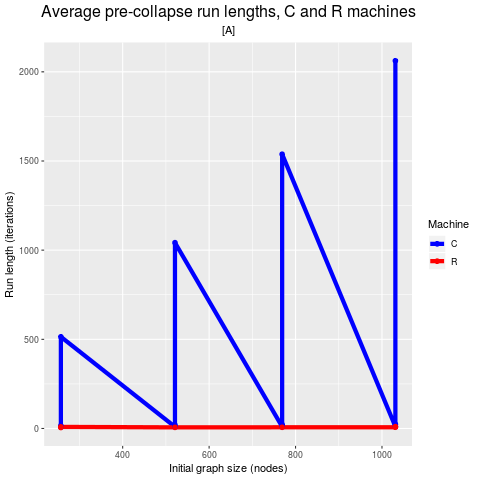
\includegraphics{figA.png}
\caption{Flows of carbon in an ecosystem.
Plants convert carbon dioxide in the atmosphere into biomass. Fungi, microbes, and animals convert plant material into soil organic matter, nutrients, and back to carbon dioxide.
Farmers who focus on selling plant material are missing out on half of the cycle.}
\end{marginfigure}

In \textit{A New Kind of Science} (199?), Stephen Wolfram methodically analyzed
a variety of cellular automata types. He found particular inspiration in the
behavior of a one-dimensional machine running "Rule 110." Among his observations were... (list
irreducibility, etc.)

Wolfram and others have also suggested that some natural processes that were
previously thought to evolve by natural selection are instead
manifestations of things that nature found "easy" to accomplish using
the same fundamental principles that underlie simple automata.

In this work, we analyze simple graph automata -- machines that operate on the same principles as
cellular automata, but use a graph, rather than a "tape" or grid, as a substrate.
Where cellular machines define cell adjacency spatially, our machines use graph topology.

\subsection{The Fungal Life Cycle: Spores, Hyphae, and Mushrooms}

\begin{marginfigure}
\includegraphics{crw-mushroom-lifecycle}
\caption{The stages of a mushroom's life. "Farming the Woods"}
\end{marginfigure}

\newthought{Mushrooms are the reproductive structure produced by some fungi}. 
Fungi spend most of their lives as hyphae - a white mass tubular chain of cells that explore the soil, wood, or other substrate and release enzymes decomposing enzymes to convert it into food and air. 
Under the right conditions - for example when the fungus is running out of food or the weather becomes favorable for finding new substrate, the fungus will form a mushroom.
It is important to note that fungi have evolved to respond to specific environmental cues - the depletion of a food source coupled with particular changes in temperature and moisture availability. 
The mushroom raises into the air, and develops gills spores into the air so that once released, they will blow in the wind, and a few lucky ones will find a new home, and germinate.
Once the spores germinate, they begin to grow as hyphae, long thin chains of cells that explore and decompose wood, and find compatible hyphae to mate.

\subsection{Spawn}

\begin{marginfigure}
\includegraphics{shiitake-spawn}
\caption{How mushroom spawn is made. First, tissue is removed from the mushroom fruitbody and transferred to  sterile culture. Then it is inoculated on a mixture of sawdust, wheat bran, and gypsum. Once the sawdust is colonized, it can be transferred to other logs. From "Farming The Woods" by Mudge and Gabriel.}
\end{marginfigure}

Spawn is a large mass of fungal hyphae grown on sawdust supplemented with a nitrogen source, commonly wheat bran. 
By growing on this sawdust, the fungus can increase its mass and growth rate. Once the sawdust is colonized, it is ready to transfer onto our logs.
The hyphae are transferred during this time of active growth  - if left too long, they will begin to loose their vigor and then fruit. 
Spawn should be purchased within a few weeks of inoculation, and kept in a cool, dark place or a refrigerator for longer periods. 

\newthought{There are Cold, Warm, and Wide climate range strains of Shiitake.}
Strains can be categorized as cold-weather (<50$^{\circ}$ F), midseason (50-64$^{\circ}$F), warm-weather (>68$^{\circ}$F), and wide range strains (41-95$^{\circ}$F). 
Growing a mixture of strains can extend the growing season. 
Warm weather strains grow more quickly, while cold weather strains produce fewer but higher quality mushrooms and will continue to produce for more seasons than faster growing strains because by growing more slowly, they conserve their food resources.

Strains vary in moisture requirement, preferred wood species, mushroom size and quality, colonization rate, and climate adaptation. 
Starting with a mixture of strains not only extends the season,  but also allows the grower to identify which ones are most
suitable to the climate of your log yard as well as your management
and marketing strategy.

\section{From Trees to Logs}

\begin{marginfigure}
\includegraphics{tree-forms}
\caption{Many trees have distinctive overall shapes; the scraggly nature of this oak is typicall \href{http://www.lostrivers.ca/content/points/treeswinter.html}{lostrivers.ca}}
\end{marginfigure}

\newthought{It is best to manually harvest fresh logs from healthy trees} Machine harvested logs (as found in lumberyards) often these have bark damaged that will make logs susceptible to drying and infection. 
Logs with discoloration of the wood seen on the ends have been colonized by other fungi and should not be used because the shiitake will be fighting an uphill battle as the late comer to the competition for room on the log.
Hopefully this makes it clear that firewood is not suitable for shiitake production - it is old, dry, split, and likely already colonized.

\begin{marginfigure}
\includegraphics{oak-leaves-twigs}
\caption{The leaves of common midwest oaks are lobed; all oaks have buds clustered at the end of the twig, and have opposite branching (unlike maple and ash)  
\href{http://www.michigan.gov/dnr/0,4570,7-153-10370_12148-61306--,00.html}{Fom "Forest Foods Deer Eat", Michigan Department of Natural Resources}
}
\end{marginfigure}

\subsection{Selecting Trees}


\newthought{Oaks are recommended} when available; indeed Shiitake means "oak mushroom" in Japanese.   
Oaks are easy to recognize, even in the winter, because of the overall form, the clustered buds, alternating branches, and the presence of oak leaves on the ground.  

Other excellent trees suitable for growing Shiitake include Maple, Ironwood, Cherry, and Sweetgum.
There are many species to avoid, including Aspen, Willow, Hickory, Ash, Elm, Locust, and conifers such as fir, pine, or spruce.

\begin{marginfigure}
\includegraphics{chainsaw-safety}
\caption{Recommended safety equipment. Also note that log is balanced, so it falls easily when cut. \href{http://www.fao.org/docrep/004/ac142e/ac142e0g.htm}{FAO Asia-Pacific Forestry Commision, 1999, "Code of Practice for Harvesting in Asia-Pacific"}}
\end{marginfigure}

Thinning a forest is an ideal way to obtain logs of an appropriate size by cutting trees that are 8-12" chest height.
It is also possible to coordinate with arborists - and in regions with rapid development, contractors often appreciate help clearing land, especially the tree tops that may otherwise be on their way to the dumpster.
The branches of much larger trees are also good sources of logs.

Once you select a tree, ensure that it is healthy, with no visible rot or damaged bark.
Also check that there are no nails or wires in the tree, that the tree is straight and balanced, and that it is not windy. 
Also check that there is a clear path for the tree to fall.

\subsection{Acquiring Logs}


\newthought{Chainsaws and falling trees can be dangerous.}
This is not intended as a comprehensive guide but as an overview.
The key steps to reducing danger are to cut smaller trees, to make sure there is clear opening for the tree to fall, and to watch out for people in the path of the falling tree.


\begin{marginfigure}
\includegraphics[width=4.5cm]{uiextension-treefelling.png}
\caption{Cuts required to fell a tree. From \href{http://www.aces.uiuc.edu/vista/html_pubs/saw/saw.html}{"Chain Saw Safety Tips", 1979, University of Illinois Extension}}
\end{marginfigure}


Logs should be cut between one to four weeks prior to inoculation, during the winter when there are no leaves. 
During this time, the logs have more carbohydrates and nutrients. 
Ideal logs for shiitake cultivation are 4-8" diameter by 3-4' long, and have few branches that need to be cut off.

After checking equipment and surroundings, it is time to start cutting.
The standard approach is to create a hinge by cutting a wedge that faces the direction of fall, followed by a back cut to create the hinge (see figure). The first cut is horizontal, and the second is at an angle. The third, or back cut, horizontal on the 

\section{Inoculating Logs}

\marginnote{
\textsc{Materials}
\begin{description}
\item sturdy table
\item 12mm drill bits with collar 
\item spawn plunger
\item high speed drill 
\item wax (cheas or bees)
\item propane torch, stove, or hot plate
\item aluminium labels and nails
\end{description}
}


\subsection{The Inoculation Workflow}

An inoculation table will get covered in wax, and should allow logs to easily roll or slide down the assembly line. 
A metal cattle gates propped up on two
sawhorses work very well because they
facilitate rolling logs down the line while
allowing sawdust, spawn, and wax to drip
through. 
Labels made of small aluminum tags that can be hammered into the ends of logs are available from most mushroom supply companies (see "Sources" below), and should be marked with the strain used and date inoculated.


\begin{figure}
\includegraphics{innoculation-workflow}
\caption{Overview of steps required to inoculate logs: drilling, inoculating, and waxing. (From "Farming the Woods")}
\end{figure}

\begin{marginfigure}
\includegraphics{drill-logs}
\caption{Another setup, similar to the one  used in today's workshop. www.mushroompeople.com}
\end{marginfigure}

If available, there should be one driller, two inoculators, and one waxer.
The second inoculator can also handle miscellaneous tasks such as refilling spawn and wax.
Spawn can be placed into an old coffee can. 
Drill holes every 6" in a line down the length of the log, rotate so the next line will be 3" below, and stagger the holes to form a diamond pattern. 
A self-taping drill bit is faster because it pulls the drill into the log.
Keep the drill running the entire time it is in the hole so that it will easily come out of the wood. 
The spacing of holes is just a guide to maximize colonization rate
and minimize damage to the bark. 
Roll the log to the inoculators, who then use plungers to fill holes with spawn.
Next, the holes are waxed to prevent
drying and infection. 
Wax should be melted in a tin can, and a paintbrush or similar device is used to cover each hole with wax.
Add a label with the date of inoculatoin and strain, as this will help you to assess
when and how much shiitake are produced
by each strain.

\section{Spawn Run}

\newthought{The spawn run is when the fungus colonizes the log}, and may take six months to two years depending on strain, weather, log size and species.
This is the time when the logs are most sensitive to contamination and dessication,  either of which will reduce yields.
Proper management during the spawn run is required to prevent logs from becoming contaminated or drying out.
Shiitake can not survive if the logs get to dry, and logs that are either too dry or too wet have will be more susceptible to contamination.

After the spawn run, the logs are less susceptible to contamination because most of the wood substrate has been colonized by shiitake. 
Actively fruiting logs will be less susceptible to drying out if the soaking method described below is used to stimulate production. 

Inoculated logs should be placed in a dead stack similar to firewood, elevated from the soil by boards, bricks, or other material. 
Where logs contact soil, they will be colonized by other fungi. 
Logs should not be stacked near nor downwind of decaying wood "trash" piles that can harbor contaminant fungi.
The ideal place for these logs is in the shade, preferably an evergreen forest that provides shade throughout the winter and inhibits the growth of competitor fungi.

Logs that have a dark crust on the bark have been contaminated by Hypoxylon. 
Hypoxylon is a common indicator that logs have not been sufficiently moist.
You can also cover the logs with shade cloth or pine branches to slow evaporation.


\begin{figure}
\includegraphics{dead-stack}
\caption{Logs placed in a 'dead stack' like firewood for spawn run. This configuration prevents drying out. Logs should not be in contact the soil, and should be watered weekly if there is no rain.}
\end{figure}

During the spawn run, it is necessary to keep the conditions favorable for shiitake and unfavorable for competitors by maintaining sufficient moisture without allowing bark to stay wet for long periods. It is important during this time to maintain log moisture between 35\% and 65\%. 
If moisture level falls below 35\%, the mushroom could die.
This is absolutely critical, and for a large operation it is a good idea to monitor the weight of individual sample logs. 
During dry summers, it may be necessary to water logs every week or two; it is preferable to water thoroughly but infrequently to allow the inside to get moist and the bark to dry out and remain dry. 

Colonization can be observed as creamy whitish discoloration at the ends of the log or seen by cutting through the bark with a knife.

\newthought{Contamination reduces yield}. 
\section{Fruiting}

Forced fruiting is used to produce a consistent supply of mushrooms during the growing season. 
Although logs will fruit naturally, more intensive management increases yields and helps to maintain a consistent supply. Fruiting requires proper temperatures and moisture, and this depends on the strain.

\begin{figure}
\includegraphics{fruiting}
\caption{A fruiting cycle. During the May-Sept season, shiitake are rotated through soaking, striking, and fruiting. 
In this figure there are seven stacks, and a different stack is processed every week. Logs are moved to a soaking tank and then lined up during fruiting in a configuration that facilitates harvest.
Adding a cold weather strain (CW) can double the length of the mushroom production season from four to almost eight months.}
\end{figure}

\newthought{The soak and strike method is used to initiate fruiting}. 
Logs can be forced to fruit by extended soaking - either 48 hours under a sprinkler or 24 hours submerged in a tank (such as those used for watering livestock). 
After soaking, the logs are struck with a mallet,  taking care not to damage older logs. 
Then, logs are placed in a lean-to or other configuration that will allow easy access to pickers.
If fruiting is forced too either before the logs are fully colonized or before they have had time to recover after fruiting, total yields will suffer. 
After fruiting, logs should be given six to twelve weeks to recover before the next fruiting. 
This cycle of fruiting and resting will provide a continual supply of mushrooms.

\begin{marginfigure}
\includegraphics{shiitake-harvest}
\caption{Harvesting shiitake from logs. Mitoku Products, www.mitoku.com}
\end{marginfigure}

Within a week or two of soaking, mushrooms will begin to fruit and pinheads - small primordial mushrooms - will begin to form. These are baby mushrooms and at this stage they are susceptible to freezing or drying, which would prevent them from maturing into a saleable mushroom. 
If the air is dry, lightly mist the logs and wet the surrounding ground to increase humidity.

Depending on temperature and strain, it may take one to three weeks from initiation to harvest. 
As the mushroom approaches harvest, a heavy rain can ruin a crop by making it soggy and unpalatable. 
For this reason, it is wise to place fruiting logs in a covered location. 
During the winter or heat of the summer, logs may be moved into a climate controlled within the fruiting range of the particular strain, in a building such as a garage or shed, but the gain in yield can come at significant cost in labor, fuel, and indoor space.

\begin{marginfigure}
\includegraphics{shiitake}
\caption{Shiitake mushrooms ready for harvest. www.mykoweb.com}
\end{marginfigure}


Yield depends on many factors, some within the farmer’s control and others up to nature and chance. 
Logs allowed to fruit naturally can be expected to produce 10\% of their fresh weight in mushrooms over their productive life, which can be 3-8 years. 
Experienced and attentive growers who use force fruiting can obtain 20\% yields, and a few see 30\%. 
To convert percentages to harvestable yield, a typical 10\% conversion would produce 10 lbs of shiitake from every 100 lbs. of logs.

\subsection{Marketing}

Fresh picked shiitake should be packaged into paper or cardboard containers, but may be sold in the plastic clamshells used for berries as long as they are aerated. 
Fresh shiitake will maintain their high quality for two weeks. 
They can be rapidly sold at \$8-12\/lb. at farmers' markets and groceries, or to individuals through community supported agriculture programs. 
A pound can fill a lunch bag and for many consumers, a pound is more than they can use before they spoil. 
One approach is to sell smaller prepackaged 4 oz. containers for \$4 to maximize profit and reduce sticker shock for the customer.

Mushrooms that fruit during early spring and late fall are slow growing and develop thick cracked caps with a particularly fine taste. 
These are known as "Donko" and if correctly marketed, can be sold at a premium. 

Fresh shiitake has advantage against shiitake from other states and especially other countries. When selling to grocers, bring in some of your fresh, local, log-grown shiitake and point out the difference between what you have to offer and what they have on the shelf. 


If you grow mushrooms on logs, you will not compete directly with these because your mushrooms will be substantially thicker and flavorful.
Next time you are at your grocery store, see what the shiitake look like, and ask where they come. 
Most will be from Pennsylvania or California, and none will have the quality of a locally log grown shiitake. 
This is for two reasons. 
First, the mushrooms have traveled far, often in plastic packaging. 
Second, log-grown shiitake are thicker and sturdier than those grown commercially indoors on sawdust supplemented with wheat bran.


\marginnote[-15cm]{
\textsc{Homework:}

\textsc{Part 1:} Go to the grocery store and inspect the quality of mushrooms you see there. 
Ask the produce manager where they come from, and how long they have been on the shelf.

\textsc{Part 2:} Next time a restaurant has mushrooms on the menu referred to as "wild", or with a vague term such as "woodland" or "gourmet", ask the server - who will likely have to ask the chef - what type of mushrooms they are.
I keep a list of menu item, how the mushroom is referred to, names given upon clarification, and actual species names if I can determine them.

\textsc{Part 3:} Write up a plan to begin a shiitake operation in which you inoculate 200 logs each year. 
What are the costs and potential returns?
}

\marginnote[-6cm]{
\textsc{Further Reading}
\begin{description}
\item[Farming the Woods:] An Integrated Permaculture Approach to Growing Food and Medicinals in Temperate Forests. Mudget and Gabriel 2014.  Chelsea Green Publishing. 359p.
\item[Mycelium Running:] How Mushrooms Can Help Save the World Stamets 2011. Ten Speed Press 435p
\end{description}

\vspace{1cm}

\textsc{Sources of Spawn and Supplies}

\begin{description}
\item[The Mushroom People] The Farm, TN. %Spawn and supplies for growing a variety of mushrooms. 
www.mushroompeople.com
\item[Field and Forest Products] Mary Ellen Kozak \& Joseph Krawczyk 
%have been growing shiitake and supplying farmers with spawn for over 30 years and are very helpful in solving problems. 
www.fieldforest.net
\item[Fungi Perfecti] Paul Stamets 
%of Ted "How Mushrooms can Save the World" fame, also author of canonical books, including "The Mushroom Cultivator" and "Growing Gourmet and Medicinal Mushrooms", and "Mycelium Running". 
www.fungi.com
\end{description}

\vspace{1cm}

\emph{This handout was based on an article I originally wrote for the Carolinia Farm Stewardship newsletter, March-April 2004.}}

\end{document}
